\documentclass{article}
\usepackage{amsmath, sfmath, multicol, tkz-euclide, array, enumerate, tcolorbox, tabularray}
\renewcommand{\familydefault}{\sfdefault}
\setlength{\parindent}{0cm}
\pagestyle{empty}
\usepackage[left=1in, top=0.5in, right=1in, bottom=0.5in]{geometry}
\tikzset{>=stealth, label style/.append style={font=\footnotesize}}
\tcbset{colback=white}

\newcounter{example}[section]
\newenvironment{example}[1][]{\refstepcounter{example}\par\medskip
   {\color{red}\textbf{Example~\theexample. #1}}}{\medskip}

\begin{document}

\section*{Trapezoids and Kites}

\begin{tcolorbox}[colframe=orange!70!white, coltitle=black, title=\textbf{Today I Can}]
\begin{enumerate}
    \item Verify and use properties of trapezoids and kites.
\end{enumerate}
\end{tcolorbox}
\bigskip 

\begin{tcolorbox}[colframe=black!20!white, opacitybacktitle=0.1, coltitle=black, title=\textbf{Trapezoid}]
A quadrilateral with only one pair of parallel sides \newline 

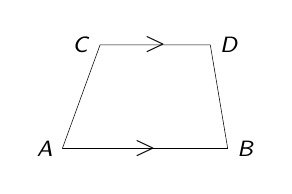
\begin{tikzpicture}[scale=0.35]
\tkzDefPoints{0/0/A, 6/0/B}
\tkzDefShiftPoint[A](70:4){C}
\tkzDefShiftPoint[C](0:4){D}
\tkzDrawPolygon(A,B,D,C)
\tkzLabelPoints[left](A,C)
\tkzLabelPoints[right](B,D)
\tkzDefMidPoint(A,B)    \tkzGetPoint{z}
\tkzDefMidPoint(C,D)    \tkzGetPoint{x}
\node at (z) {$>$};
\node at (x) {$>$};
\end{tikzpicture}
\end{tcolorbox}

\begin{tcolorbox}[colframe=black!20!white, opacitybacktitle=0.1, coltitle=black, title=\textbf{Isosceles Trapezoid}]
A trapezoid with congruent non-parallel sides (called \textit{legs}). \newline 

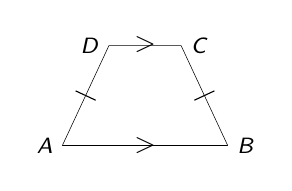
\begin{tikzpicture}[scale=0.7]
\tkzDefPoints{0/0/A, 3/0/B}
\tkzDefShiftPoint[A](65:2){D}
\tkzDefShiftPoint[B](115:2){C}
\tkzDrawPolygon(A,B,C,D)
\tkzLabelPoints[left](A,D)
\tkzLabelPoints[right](B,C)
\tkzMarkSegments[mark=|](A,D B,C)
\node at (1.5,0) {$>$};
\node at (1.5,1.825) {$>$};
\end{tikzpicture}
\end{tcolorbox}

\begin{example} \label{isos_trap}
$CDEF$ is an isosceles trapezoid. What are the measures of the other angles? \newline

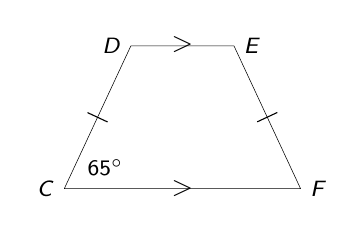
\begin{tikzpicture}
\tkzDefPoints{0/0/C, 3/0/F}
\tkzDefShiftPoint[C](65:2){D}
\tkzDefShiftPoint[F](115:2){E}
\tkzDrawPolygon(C,F,E,D)
\tkzLabelPoints[left](C,D)
\tkzLabelPoints[right](E,F)
\tkzLabelAngle[pos=0.5,xshift=0.1cm](F,C,D){\footnotesize $65^\circ$}
\tkzMarkSegments[mark=|](C,D E,F)
\node at (1.5,0) {$>$};
\node at (1.5,1.825) {$>$};
\end{tikzpicture}
\end{example}

\begin{example}
In the diagram $PQRS$ is an isosceles trapezoid. What are the measures of the other angles?
\newline\\

\begin{tikzpicture}
\tkzDefPoints{0/0/Q, 0/-3/P}
\tkzDefShiftPoint[P](16:2){S}
\tkzDefShiftPoint[Q](-16:2){R}
\tkzDrawPolygon(P,Q,R,S)
\tkzLabelPoints[below](P,S)
\tkzLabelPoints[above](Q,R)
\tkzMarkSegments[mark=|](Q,R P,S)
\tkzLabelAngle[pos=-0.5](S,R,Q){\footnotesize $106^\circ$}
\end{tikzpicture}
\end{example}

\begin{example}
In Example \ref{isos_trap}, if $CDEF$ were not an isosceles trapezoid, would $\angle C$ and $\angle D$ still be supplementary? Explain.
\end{example}

\begin{tcolorbox}[colframe=black!20!white, opacitybacktitle=0.1, coltitle=black, title=\textbf{Midsegment of a Trapezoid}]
A segment that joins the midpoints of the legs.\newline 

\begin{minipage}{0.5\textwidth}
\begin{itemize}
    \item $\overline{AB} \parallel \overline{EF} \parallel \overline{CD}$
    \item $EF = \frac{1}{2}\left(AB + CD\right)$
\end{itemize}
\end{minipage}
\begin{minipage}{0.4\textwidth}
    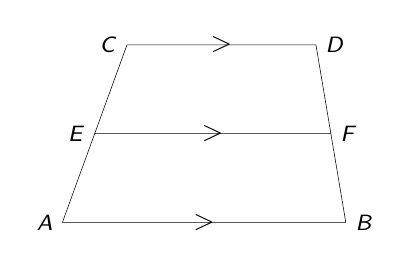
\begin{tikzpicture}[scale=0.6]
    \tkzDefPoints{0/0/A, 6/0/B}
    \tkzDefShiftPoint[A](70:4){C}
    \tkzDefShiftPoint[C](0:4){D}
    \tkzDrawPolygon(A,B,D,C)
    \tkzDefMidPoint(A,C)    \tkzGetPoint{E}    
    \tkzDefMidPoint(B,D)    \tkzGetPoint{F}
    \tkzDrawSegment(E,F)
    \tkzLabelPoints[left](A,E,C)
    \tkzLabelPoints[right](B,F,D)
    \tkzDefMidPoint(A,B)    \tkzGetPoint{z}
    \tkzDefMidPoint(E,F)    \tkzGetPoint{y}
    \tkzDefMidPoint(C,D)    \tkzGetPoint{x}
    \node at (z) {$>$};
    \node at (y) {$>$};
    \node at (x) {$>$};
    \end{tikzpicture}
\end{minipage}
\end{tcolorbox}

\begin{example}
Find the value of $x$ and the length of the midsegment in each.
\begin{multicols}{2}
\begin{enumerate}[(a)]
    \item \mbox{}
    \item \mbox{}
\end{enumerate}
\end{multicols}
\begin{minipage}{0.5\textwidth}
    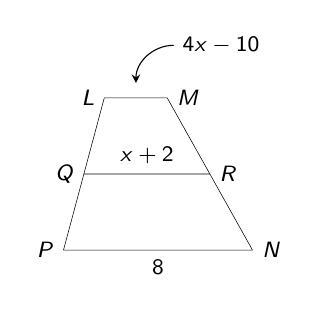
\begin{tikzpicture}[scale=0.8]
    \tkzDefPoints{0/0/P, 3/0/N}
    \tkzDefShiftPoint[P](75:2.5){L}
    \tkzDefShiftPoint[L](0:1){M}
    \tkzDrawPolygon(P,L,M,N)
    \tkzDefMidPoint(P,L)    \tkzGetPoint{Q}
    \tkzDefMidPoint(M,N)    \tkzGetPoint{R}
    \tkzDrawSegment(Q,R)
    \tkzLabelPoints[left](P,Q,L)
    \tkzLabelPoints[right](M,R,N)
    \tkzLabelSegment[below](P,N){8}
    \tkzLabelSegment[above](Q,R){\footnotesize $x+2$}
    \node at (2.5,3.25) {\footnotesize $4x-10$};
    \draw [->, >=stealth] (1.75,3.25) arc (90:180:0.6cm);
    \end{tikzpicture}
\end{minipage}
\begin{minipage}{0.4\textwidth}
    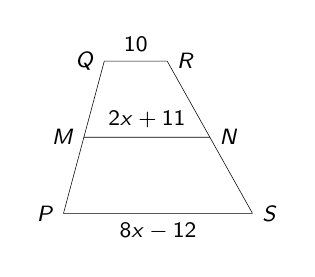
\begin{tikzpicture}[scale=0.8]
    \tkzDefPoints{0/0/P, 3/0/S}
    \tkzDefShiftPoint[P](75:2.5){Q}
    \tkzDefShiftPoint[Q](0:1){R}
    \tkzDrawPolygon(P,Q,R,S)
    \tkzDefMidPoint(P,Q)    \tkzGetPoint{M}
    \tkzDefMidPoint(R,S)    \tkzGetPoint{N}
    \tkzDrawSegment(M,N)
    \tkzLabelPoints[left](P,Q,M)
    \tkzLabelPoints[right](S,R,N)
    \tkzLabelSegment[below](P,S){\footnotesize $8x-12$}
    \tkzLabelSegment[above](M,N){\footnotesize $2x+11$}
    \tkzLabelSegment[above](Q,R){10}
    \end{tikzpicture}
\end{minipage}
\end{example}

\vfill 

\begin{tcolorbox}[colframe=black!20!white, opacitybacktitle=0.1, coltitle=black, title=\textbf{Kite}]
A quadrilateral with 2 pairs of consecutive sides congruent and no opposite sides congruent. \newline 

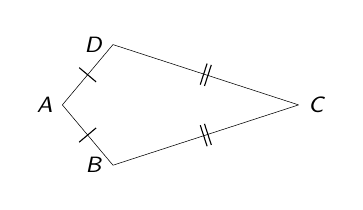
\begin{tikzpicture}[scale=0.5]
\tkzDefPoints{0/0/A, 6/0/C}
\tkzDefShiftPoint[A](-50:2){B}
\tkzDefShiftPoint[A](50:2){D}
\tkzDrawPolygon(A,B,C,D)
\tkzLabelPoints[left](A,B,D)
\tkzLabelPoints[right](C)
\tkzMarkSegments[mark=|](A,D A,B)
\tkzMarkSegments[mark=||](C,D C,B)
\end{tikzpicture}
\end{tcolorbox}

\begin{example}
Find the measures of the numbered angles in each kite.
\begin{multicols}{2}
\begin{enumerate}[(a)]
    \item \mbox{} 
    \item \mbox{}
\end{enumerate}
\end{multicols}
\begin{minipage}{0.5\textwidth}
    \begin{tikzpicture}[scale=0.8]
    \tkzDefPoints{0/0/E, 3.5/0/G, 1.75/1.5/D, 1.75/-2.5/F}
    \tkzDrawPolygon(E,D,G,F)
    \tkzDrawSegments(D,F E,G)
    \tkzLabelPoints[left](E)
    \tkzLabelPoints[below](F)
    \tkzLabelPoints[above](D)
    \tkzLabelPoints[right](G)
    \tkzLabelAngle[pos=0.8](F,D,G){\footnotesize $52^\circ$}
    \tkzLabelAngle[pos=0.5](E,D,F){\footnotesize 3}
    \tkzLabelAngle[pos=0.6](E,G,D){\footnotesize 2}
    \node at (1.75,0) [anchor = south west] {\footnotesize 1};
    \end{tikzpicture}
\end{minipage}
\begin{minipage}{0.4\textwidth}
    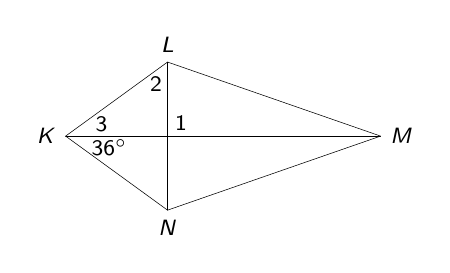
\begin{tikzpicture}[scale=0.8]
    \tkzDefPoints{0/0/K, 5/0/M}
    \tkzDefShiftPoint[K](36:2){L}
    \tkzDefShiftPoint[K](-36:2){N}
    \tkzDrawPolygon(K,L,M,N)
    \tkzDrawSegments(K,M L,N)
    \tkzInterLL(K,M)(L,N)   \tkzGetPoint{O}
    \tkzLabelPoints[left](K)
    \tkzLabelPoints[above](L)
    \tkzLabelPoints[below](N)
    \tkzLabelPoints[right](M)
    \tkzLabelAngle[pos=-0.3](K,O,N){\footnotesize 1}
    \tkzLabelAngle[pos=0.4](K,L,N){\footnotesize 2}
    \tkzLabelAngle[pos=0.6,xshift=0.1cm](N,K,M){\footnotesize $36^\circ$}
    \tkzLabelAngle[pos=0.6](M,K,L){\footnotesize 3}
    \end{tikzpicture}
\end{minipage}
\end{example}

\vfill 

\end{document}
